\section{Acknowledgment}
I would like to thank Mr. Christian Motz, the Director Legal/HR at Favendo GmbH, for giving me the opportunity to do an internship within the organization. I would also like to convey my sincere gratitude to my former supervisor Mr. Stephan Lemnitzer and Mr. Lukas A. Schwoebel for a rewarding learning opportunity with them.

\section{Introduction}
I have participated in an internship program offered by Favendo GmbH \cite{favendoataglance} in Bamberg for four months starting from April 2018 and concluding on July 2018. Favendo is a software company established on 2014 with development sites mainly in Bamberg and Jena in Germany, provides cutting edge Location Based Services to its internationally spread customer base. Favendo is also part of Fewclicks corporate group \cite{fewclicksataglance} which closely deals with Web Application Services and Internet of Things based solutions. Favendo has provided location based services and solutions to customers from various demographics. Some of the prominent examples are Audi AG, SAP and Mediterranean Shipping Company cruise ships. This internship is part of my ongoing masters program at University of Bamberg in Germany. I would like to start with introducing briefly, the core services and solutions offered by Favendo.

\par Core services offered by Favendo can be divided into several categories as referred from the Favendo Official references \cite{favendoataglance}:
\begin{itemize}
	\item \textbf{WayFinding}
	\par Way finding and indoor navigation is one of the Favendo key services that is offered with the help of hardware components such as BLE beacons and a mobile software framework, in conjunction with a highly available backend server component. This service helps the users in finding their navigation path from a given source to destination at the indoor venues such as airport, shopping malls or large cruise ships with hand-held  smart devices. A high degree of accuracy helps in precisely locating a point of interest in large complex venues. Normally, a combination of several technologies such as low energy consuming crypto-beacons along with core development framework of popular software ecosystems are used to bring the solution to the customer.
	\begin{figure}[H]
		\centering
		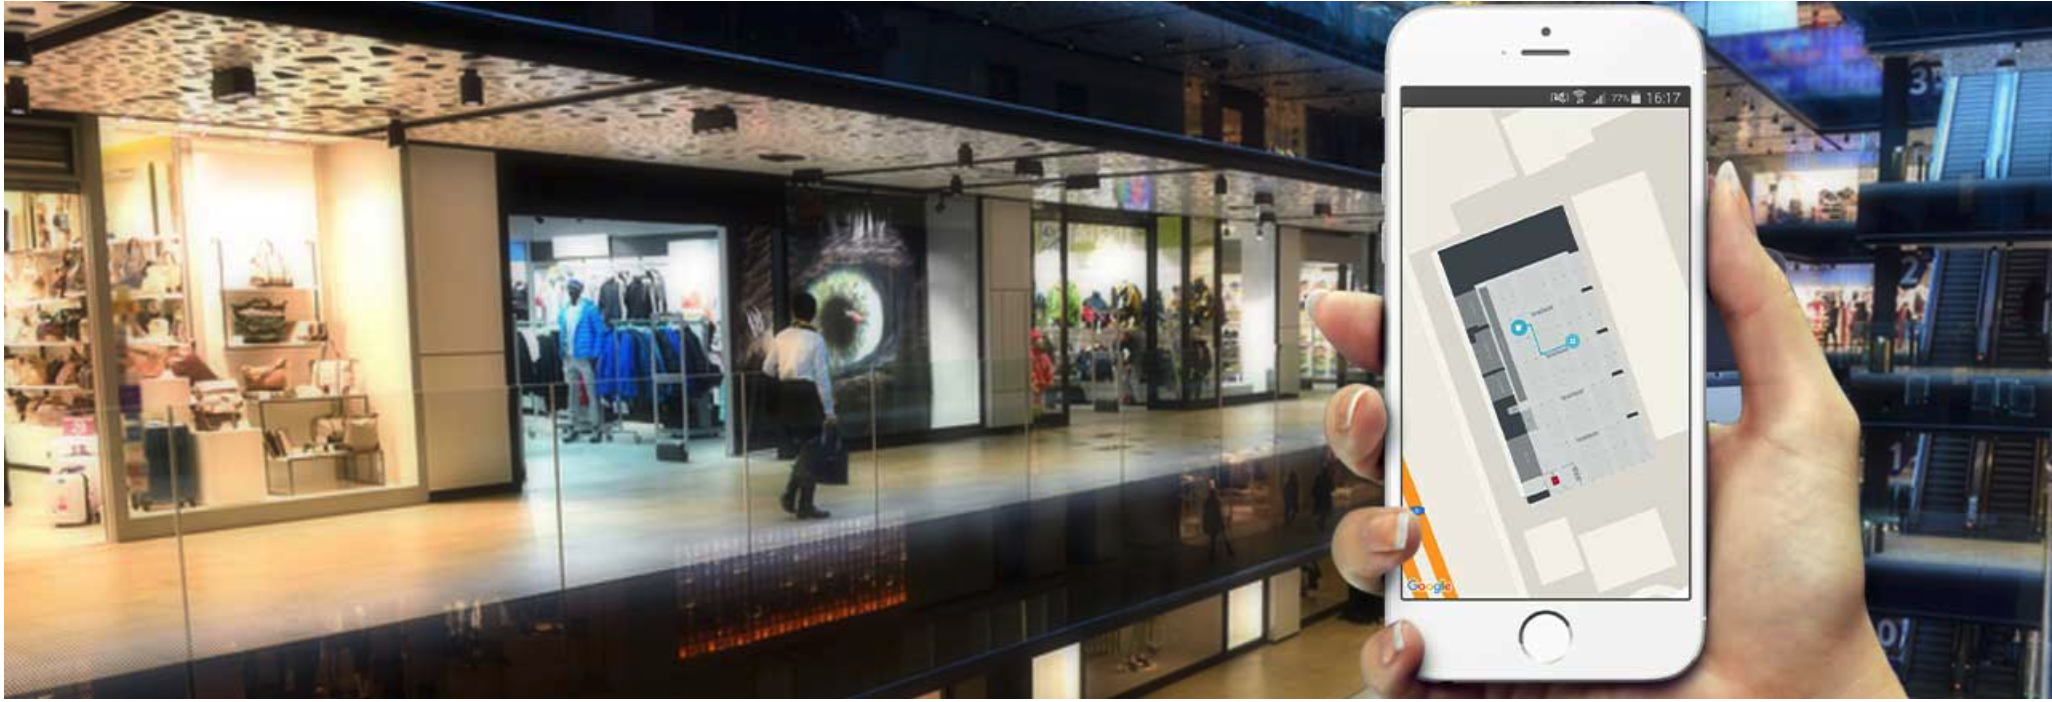
\includegraphics[scale = 0.3]{images/wayfinding}
		\caption{Way Finding sample application from Favendo Official \cite{favendoataglance}}
		\label{figure:wayfinding_sample}
	\end{figure}
	\par WayFinding carries value both for external visitors as well as the authority using the Favendo provided solution. On one hand visitors can find their way to desired destination in a large building or complex. On the other hand, respective authorities can use visitors data through analytics and use the same for proximity marketing and many other thoughtful purposes in order to boost the business.
	\item \textbf{Asset Tracking}
	\par Asset Tracking was always been a challenge worth considering for large industries, especially in sectors like construction, hospital management or large recreational venues like cruise ships. It is crucial to search items of interest in the hour of need and ensure security for them. Asset Tracking system developed by Favendo can be helpful in tracking the positions/potential utilizations of equipments or in certain cases even human beings. It is far more than just keeping track of matters. It could also be helpful in routing and smart arrival/availability predictions.
	 \begin{figure}[H]
	 	\centering
	 	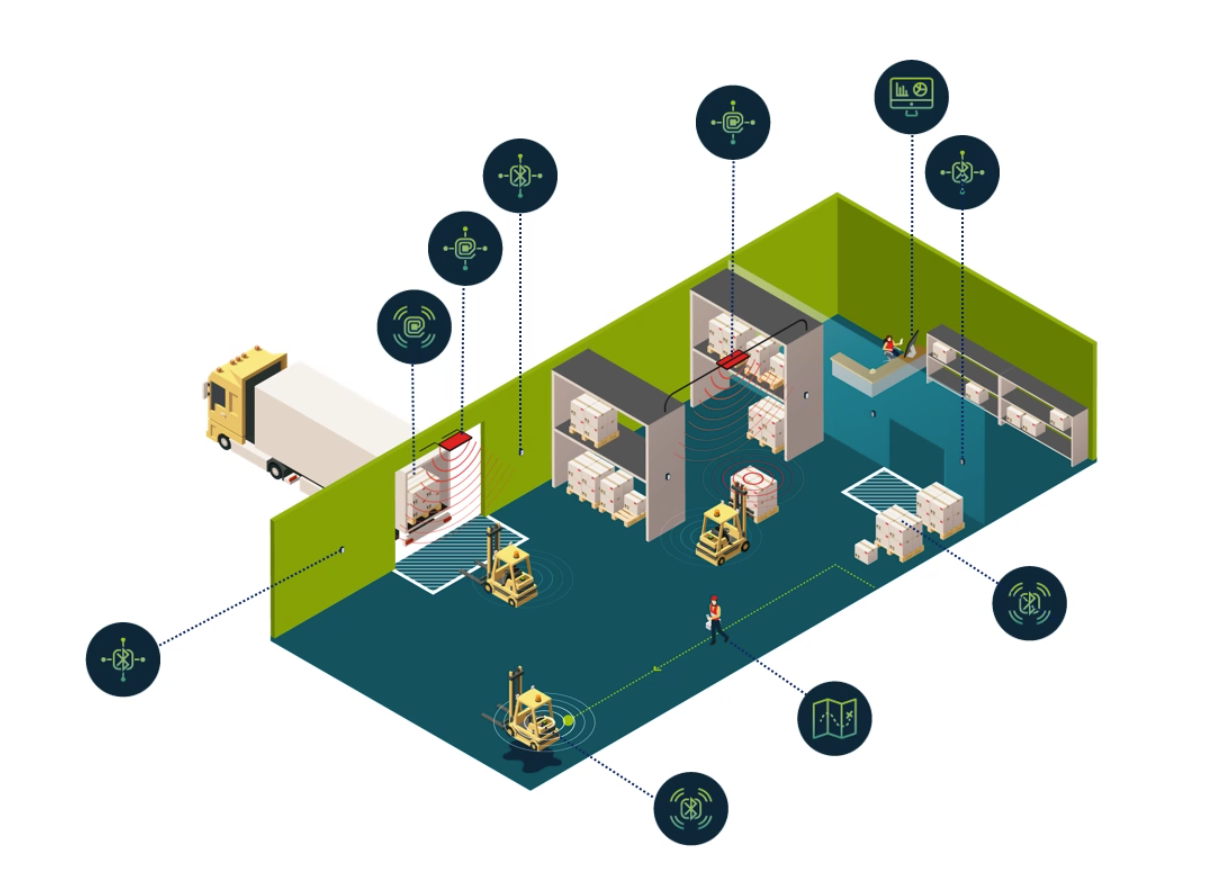
\includegraphics[scale = 0.3]{images/assettracking}
	 	\caption{Asset Tracking concept from Favendo Official \cite{favendoataglance}}
	 	\label{figure:assettracking_concept}
	 \end{figure}
	 \par Favendo offers hardware/asset tags based on crypto-beacons and RFID technology as well as a software framework that goes hand in hand in order to create an Internet of Things based real time implementation of Asset Tracking. Use of bluloc \cite{blulocfavendo} crypto-beacons makes a durable installation of signal radiators which are intercepted by beacon controllers and analyzed by the software systems to generate useful knowledge.
	 \item \textbf{Proximity Marketing}
	 \par Proximity Marketing has introduced a new paradigm of customer engagement for the businesses in order to improve sales. The key idea of the proximity marketing often relies upon the accurate positioning systems in place and it exposes unprecedented opportunities to improve business as a whole. Proximity marketing can be utilized to reach customers with making venue-specific products or offers information available.
	 \begin{figure}[H]
	 	\centering
	 	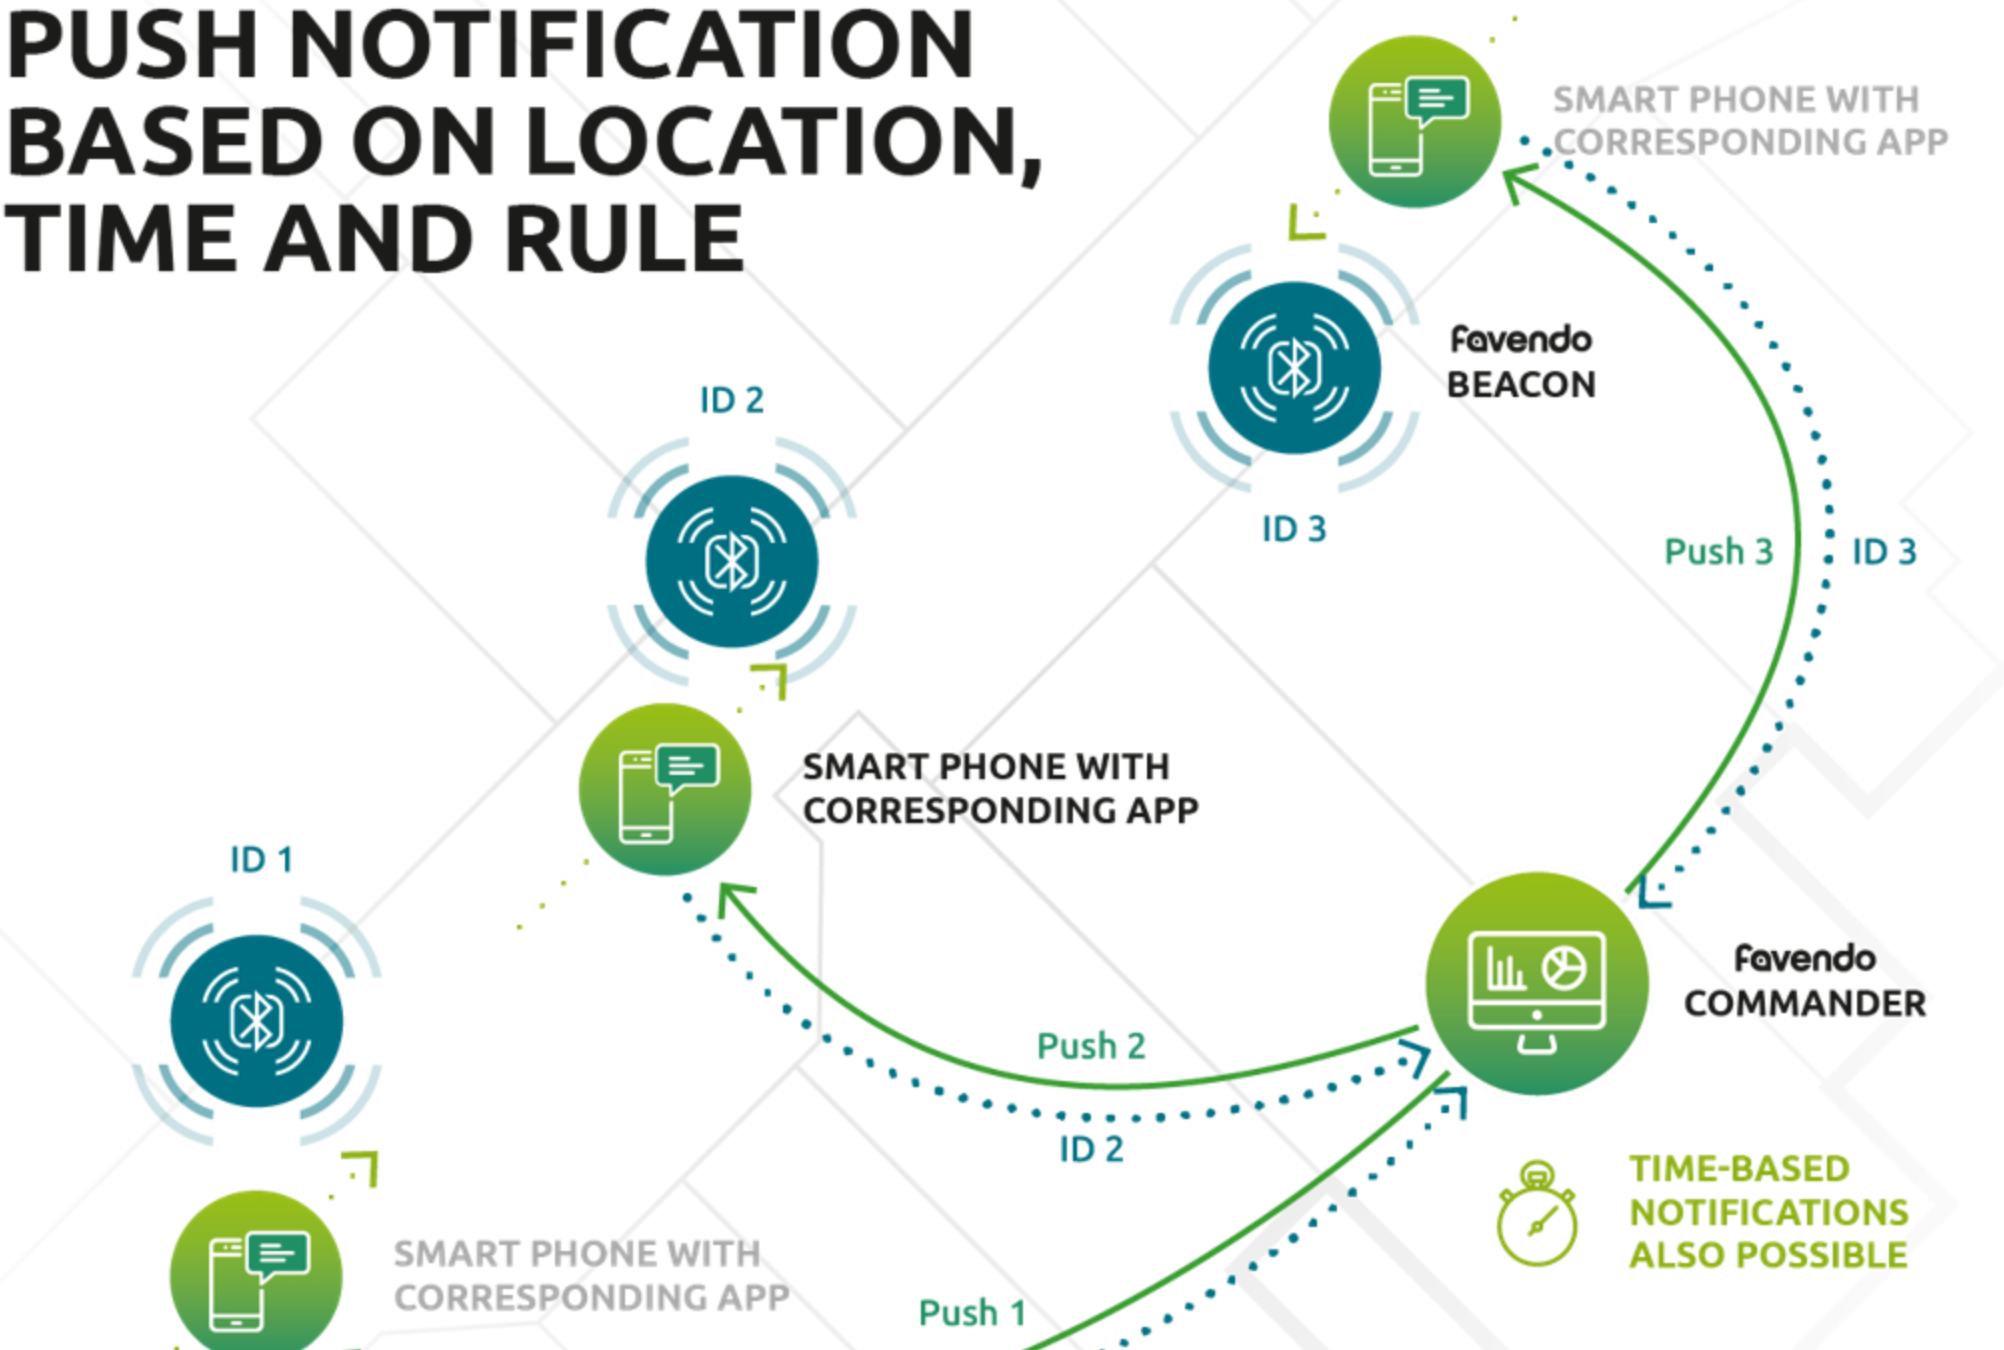
\includegraphics[scale = 0.25]{images/proximitymarketting}
	 	\caption{Proximity Marketing concept from Favendo Official \cite{favendoataglance}}
	 	\label{figure:proximitymarketing_concept}
	 \end{figure}
 	\par We can assume a very simple use case of making the content or commercial offers available in mobile devices of potential customers when they enter a specific zone or in close vicinity with the point of interest. The solution offered by Favendo is implemented with beacons making it independent of the network connectivity.
 	\item \textbf{Analytics}
 	\par Analytics utility is built in within the web based dashboard application that Favendo offers to its customers. This datasets covers a wide range such as the purchasing trends, navigation patterns or interactions with tracked objects or assets.
 	\begin{figure}[H]
 		\centering
 		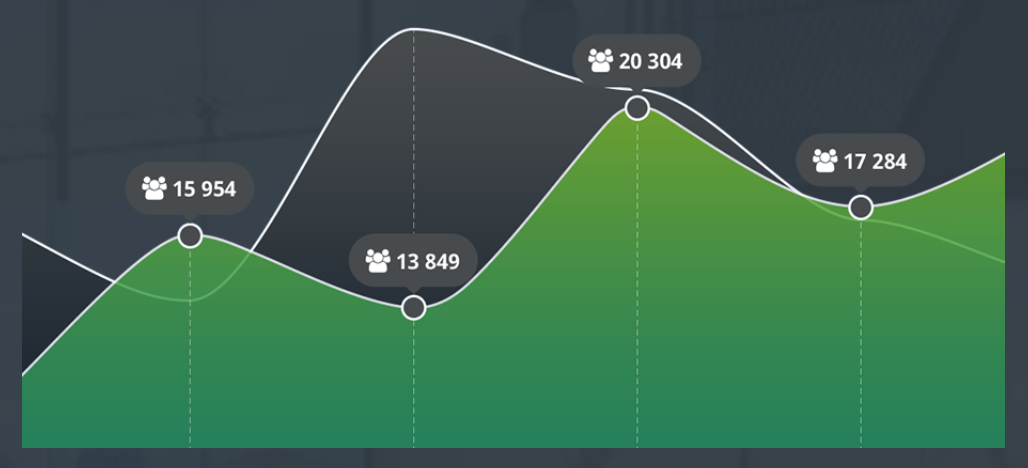
\includegraphics[scale = 0.5]{images/analytics}
 		\caption{Analytics concept from Favendo Official \cite{favendoataglance}}
 		\label{figure:analytics_concept}
 	\end{figure}
 	\par This invaluable dataset could help customers with determining the possible optimization scopes in their product lines or services offered as well as taking rational decisions improving the customer engagement. The image \ref{figure:analytics_concept} shows a concept study made for an indoor shopping center to have an overall idea of visitors movement over a course of time.
\end{itemize}

\par Since my internship was in context of software systems science, In the next sections I would provide a humble introduction of the software frameworks I have dealt with along with an illustration of the activities I was engaged with.

\subsection{Description}
Efficient framework system plays a key role in the services that Favendo offers to its customers and works as the enabler and customization point for consuming location based service. It consists of several related subsystems and goes by the project name Commander \cite{commanderfavendo}. Commander is executed with a highly available backend server side module that often securely hosts the classified information and a highly customizable mobile application SDK that is used to integrate location based services offered by Favendo to the mobile application developed for popular mobile software ecosystems such as iOS an Android. In order to provide the indoor navigation/positioning utility this framework comes with a map implementation customizable as per specific customer needs.

\par During my internship I was engaged with various enhancements and bug-fixes for this framework especially applicable for the iOS mobile platform. I have participated in the research and development efforts targeted towards the next major release of the commander mobile framework. I have learned a great deal about the iOS ecosystem in general and application programming constructs and relevant design patterns both with Swift and Objective-C as programming languages. I have participated in development efforts of reusable frameworks in the mobile application development. In the next sections I have provided a vivid summary of the subject matters that I have learned or closely dealt with and my reflection of the same.
\subsection{Key Concepts and Activities}
In this section I would like to illustrate the subject  matters that formed the core of my internship and the concepts I have dealt with.

\subsubsection{Object Oriented Programming and Design Patterns}
M. D. Smith et al. \cite{smith2011object} have described the object oriented design paradigm as the specification of task to be performed in terms of the associated objects and properties/behaviors of the objects. They have further illustrated an object as an instantiated entity having some operations it is capable to respond. It has state which could be impacted by the associated operations. Objects can invoke operations of other objects by passing messages. Smith et al. \cite{smith2011object} has also described a class as an interface specifying the properties and behaviors of an object. Properties defined inside the class determines the state of the object when instantiated. OOP paradigm provides abstraction and encapsulation contributing to security and modularity the real power of re-usability comes in the form of inheritance. OOP has contributed in developing maintainable code for many large and sophisticated software applications. 
\par Despite the capabilities that OOP has offered, modern software development can not be realized without adherence of appropriate architecture and design paradigm which needs us to adhere to certain disciplines while writing software application code. Erich Gamma et al.(The Gang of Four) \cite{gamma1995design}  have mentioned that design patterns are the mechanism to identify, name and abstract away common themes in object oriented designs. They are generally based on the intent behind the design and they identify the collaboration, rolls and responsibilities of different objects in building a software application or solution. A very common frequently used example in mobile applications demographic is Model View Controller(MVC) design pattern which is often referred from the development of  Smalltalk-80 programming environment as illustrated in the work of Krasner et al. \cite{krasner1988description}. The key focus of the MVC design patterns is to separate the functional units of an application for modularity and easier maintenance. It separates the class instances encapsulating data and operations related to the application domain as \texttt{Model}, the presentation and display of the application state as \texttt{View} and user interaction and response with the model and the view as \texttt{Controller}. MVC is one of the popular design patterns often realized while developing standalone mobile applications. While there are many popular design patterns, in my internship I have worked with three popular object oriented design patterns as briefly illustrated below.
\begin{itemize}
	\item \textbf{Mediator}
	\par The Gang of Four \cite{gamma1995design} describes the Mediator design pattern with an object that encapsulates the cooperation and interactions between several other objects by preventing them refer to each other explicitly. Object orientation suggests to reasonably distribute the application behavior among several objects. But since often one object needs to interact with other objects in the object oriented design it may result in many interconnection among the objects. While this distribution of responsibilities makes the system modular but uncontrolled interconnection and interdependencies makes the system appears as monolithic.
	\begin{figure}[H]
		\centering
		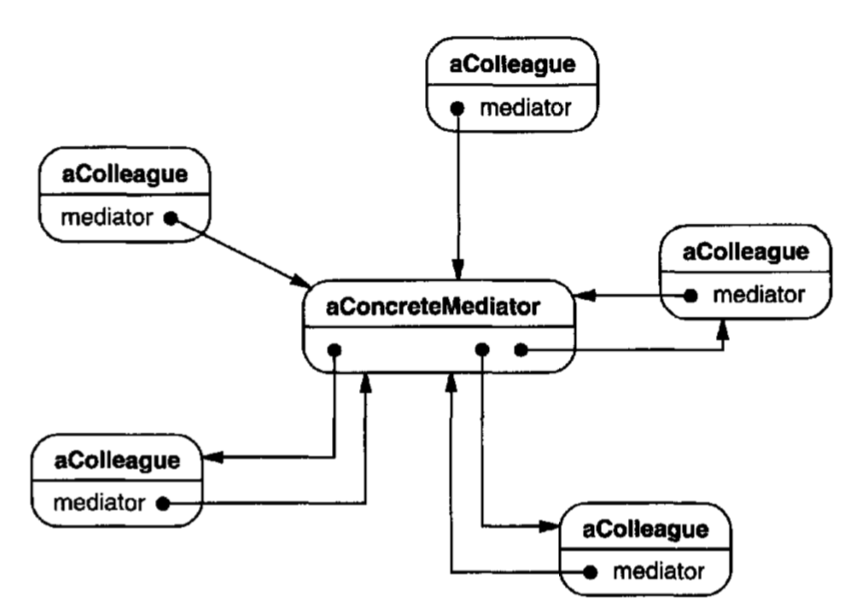
\includegraphics[scale = 0.5]{images/mediator}
		\caption{Generic Mediator diagram as explained by The Gang of Four  \cite{gamma1995design}}
		\label{figure:design_pattern_mediator}
	\end{figure}
	\par We can assign such collective behavior to a mediator object and let it coordinate among a group of objects and serve as an intermediary. The individual objects only know the mediator, resulting in reduced interconnection. In the diagram \ref{figure:design_pattern_mediator} we have  \texttt{aConcreteMediator} type acting as an intermediary among the several objects often referred as \texttt{aColleague} as per The Gang of Four \cite{gamma1995design}. Favendo Commander framework has several individually shippable modules responsible for various tasks aiding location based services. We have used Mediator design pattern to coordinate among these modules in the next release of the framework in order to create an complete service provided by the framework.
	\item \textbf{Strategy}
	\par The Gang of Four \cite{gamma1995design} defines the Strategy design pattern as the capability of encapsulating  a family of algorithms and making them interchangeable. In essence for different clients that are going to use the algorithm we can easily swap one strategy for other as per the clients needs and the underlying algorithm would also differ accordingly.
	\begin{figure}[H]
		\centering
		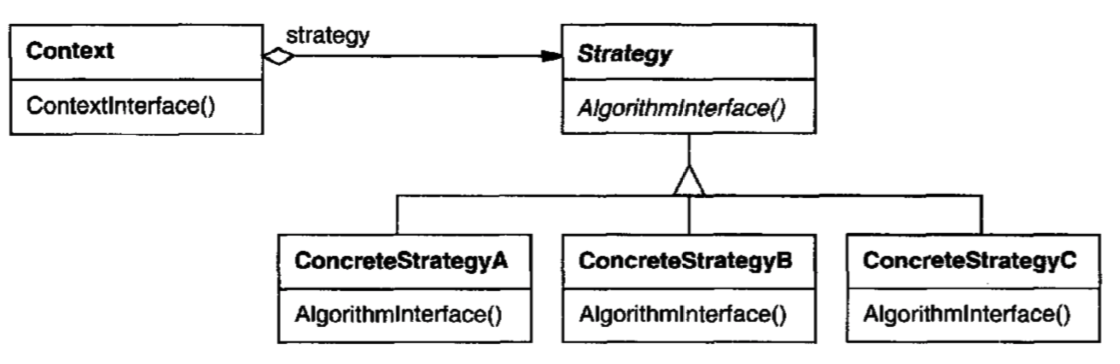
\includegraphics[scale = 0.5]{images/strategy}
		\caption{Generic Strategy diagram as explained by The Gang of Four  \cite{gamma1995design}}
		\label{figure:design_pattern_strategy}
	\end{figure}
	\par Strategy often also called Policy design pattern, is applicable when several related objects having commonalities, only differs in certain behavior at runtime. In the basic structure \ref{figure:design_pattern_strategy} provided by The Gang of Four \cite{gamma1995design} we see that \texttt{Context} refers to the object that exposes a common interface which has a reference to a \texttt{Strategy} which could be an abstract base type or a protocol in certain languages. And we have several child types e.g. \texttt{ConcreteStrategyA} \texttt{B} and so on which derive from base type \texttt{Strategy}. From the perspective of \texttt{Context} it only has a strategy to carryout some task. Depending on the requirement, we can swap one child type for other in order to provide different outcomes for different strategies. Often in our framework in concern, we needed to record the specifications received from beacons hidden in a given zone in order to measure the outcome from our positioning algorithms. We could use different serialization strategies for these recording and we have found using strategy design pattern in this regard makes the implementation cleaner.
	\item \textbf{Delegate}
	\par Delegation as the Swift documentation \cite{swiftdelegation} illustrates, is a design pattern that features an object to hand over certain responsibilities to another object. So the later becomes so called delegate of the former. Wikipedia reference \cite{wikidelegation} on delegation describes it in a more general sense such that delegation is defined by the evaluation of some properties by one object(delegate) in the context of another (sender). Delegation is a useful design pattern in OOP and its implementation can be observed throughout the software ecosystems designed by Apple e.g iOS, watchOS, tvOS, macOS and even its predecessor NextStep as mentioned in \cite{wikidelegation}.
	\par Delegation is relatively simple design pattern and often contributes a great deal to achieve a clean code in software applications. Particularly in Apple software ecosystems, specifically in the languages like Objective-C and Swift, delegate pattern is implemented using a language construct called \texttt{protocol} \cite{wikidelegation} which is analogous to interfaces in other languages like Java. In our framework we have made use of delegate pattern extensively in order to achieve a cleaner object to object interactions as it is prescribed by Apple.
\end{itemize}
Below \ref{table:design_patterns} is a summary of the design patterns that I have implemented in my work during my internship.

\begin{longtable}{|| c | p{.70\textwidth} |} 
	\hline
	\textbf{Design Pattern} & \textbf{Specification} \\ \hline
	\textbf{Mediator} & 
	\begin{itemize}
		\item Defines an object that determines how several other objects should interact and inter-operate.
		\item Enables loose coupling in complex objects orchestration.
	\end{itemize}
	\\ \hline
	\textbf{Strategy} &
	\begin{itemize}
		\item Defines a set of interchangeable algorithms with commonalities.
		\item Decouples the use of algorithms from their users.
	\end{itemize}
	\\ \hline
	\textbf{Delegate} & 
	\begin{itemize}
		\item Enables combination of simple objects into complex object system and code reuse.
		\item Promotes cleaner code.
	\end{itemize}
	\\ \hline
	\caption{Summary of design patterns dealt with \cite{gamma1995design}}
	\label{table:design_patterns}
\end{longtable}

\subsubsection{Test Driven Development}
Wikipedia \cite{wikitdd} defines TDD as the software development paradigm based on repeating shorter development cycles. The required outcome of a standalone program/application or a framework is broken into specific test cases first and then the code implementation is written to pass the tests. TDD inspires more confidence on the developed implementation and mitigates the chances of having bugs in the code.
\par Janzen et al. \cite{janzen2005test} have illustrated the idea of Test Driven Development into three inherent aspects.
\begin{itemize}
	\item \textbf{The Test Aspect}
	\par Janzen et al. \cite{janzen2005test} explains that the essence of TDD is to write automated tests in order to check the valid outcome often called acceptance criteria for units of a program. It is arguable in software development, what constitutes a unit of a program. Normally developers consider a method or function at the very least, as a testable unit. These unit tests could be manual process performed by the developers or could be part of continuous integration testing dealt with dedicated servers. Traditionally we are familiar with writing unit tests after so called unit or functions are coded. In the TDD discipline developers are supposed to write tests prior to write the code for implementation of the units which enables the unit tests to be executable write after they are written.
	\item \textbf{The Driven Aspect}
	\par The driven aspect is often interpreted as the practice of writing tests prior to the implementation. However Janzen et al. \cite{janzen2005test}  explains that \texttt{driven} in TDD focuses on how tests lead the analysis, design and programming decisions for the entire application or framework. Refactoring plays a key role in this driving process. Refactoring deals with making the code cleaner and simpler without affecting the outcome of the code and tests should still pass. It is often difficult practice to adhere to realize that TDD is more about design and analysis of the entire code and not about having bunch of tests passed. Often while designing APIs this test driven aspect plays a big role in defining the interface that we want to make publicly available.
	\item \textbf{The Development Aspect}
	\par Janzen et al. \cite{janzen2005test} further explains the TDD is not a software development methodology. It is practice that could be integrated with other essential practice in certain order and frequency. TDD can be realized as a micro-process in the chain/system or other software development processes. Adherence of TDD creates a set of automated test models which should be considered useless when the design decision for the software is made. Instead they should be considered a crucial component of the development process, capable ot providing quick feedback for any changes made in the code and their implications. If at any point an automated test fails, software developers get the feedback that there implementations that doesn't meet the acceptance criteria and should be considered fixing or altering.
\end{itemize}
Test Driven Development paradigm fits well in the context of iterative, incremental and evolutionary software development models. In my ongoing internship I have tried to study and apply the TDD practices in developing internal sub-frameworks aiding the capabilities of Favendo Commander master framework.

\subsubsection{Beacon Ranging and Overview of Indoor Positioning}
In accordance with the activities and concepts I have dealt with in my internship, I would illustrate this sub section the concepts of beacon ranging and positioning in terms of iBeacon specification and location aware frameworks designed by Apple. Apple introduced the iBeacon specification  with the launch of iOS 7. As per the apple official iBeacon reference \cite{appleibeacon} iBeacon technology utilizes the Bluetooth Low Energy in order to create a beacon region around an object embedded with or implemented as iBeacon technology. An iOS device can receive feedback upon entering or exiting an iBeacon region along with the estimated proximity to the beacon in terms of varying signal strength(RSSI)  values. We need to consider the both hardware and software components in order to create an iBeacon-based solution.
\par Manufacturers interested in creating iBeacon technology based hardware e.g. beacons need to obtain official license from Apple. Application developers interested in implementing location awareness in iOS application needs to make use of apple designed CoreLocation \cite{applecorelocation} framework while programming.
\par One of the key services offered by Favendo is indoor positioning which is implemented for iOS ecosystem based in iBeacon technology which specifies that each beacon will advertise a 16 bytes unique identifier \texttt{UUID} for the region and 2 bytes numeric \texttt{major} and \texttt{minor}  values in order subdivide a given physical location in different regions to aid the positioning. Besides in order to provide an estimated proximity from a beacon the CoreLocation framework defines some enumeration values which in turn encapsulates a range of RSSI values underneath. Only challenge the method poses is that iOS devices get feed of fluctuating signal strength coming from the iBeacon in every second and we need smoothing algorithm in order to filter out some RSSI values and consider the ones which could give us with a considerable approximation of the position of the device in given indoor location. One of the efficient ways to achieve this is to use Kalman filtering algorithm also known as Linear Quadratic Estimation as per Wikipedia reference \cite{wikikalmanfilter}. 
\par Kalman filtering algorithm relies on a series of measurements observed over time having some sort of inaccuracies and it derives estimates overtime which are better and more accurate than the estimates based on single measurements alone. Grewal et al. \cite{grewal2011kalman} have regarded Kalman filtering algorithm as a greater discovery in the filed of statistical estimation. In my internship I have designed framework which can range iBeacons and records them in serialized formats. These recording include a patterns of the signal strength values received from one of several beacons in certain location overtime as we navigate through a given location. We feed these recording to our positioning algorithms to test the outcome which gives us a measure of accuracy of the algorithms and helps us to fix the anomalies and optimize for better estimation.
